\documentclass[ignorenonframetext]{beamer}
\usetheme{Pittsburgh}
\setbeamercolor{normal text}{bg=red!7}
\usepackage{amsmath,amssymb,graphicx}
\DeclareGraphicsRule{*}{mps}{*}{}
\graphicspath{{../}}
\newfont{\normald}{logod10 scaled 1024}
\newcommand{\MF}{{\normald METAFONT}}
\newcommand{\MP}{{\normald METAPOST}}
\newcommand{\FP}{{\normald FEATPOST}}
\newcommand{\myem}[1]{\texttt{#1}}
\begin{document}

\frame{
  \frametitle{\myem{intersectorus}( $\vec{c}$, $\vec{M}$, $R_B$, $R_s$, $\vec{p}$, $\vec{D}$ )}
  \begin{center}
    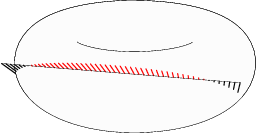
\includegraphics[width=80mm]{intersectorus.1} 
  \end{center}
}

\end{document}

